\chapter{Arhitektura i dizajn sustava}
		
		\textbf{\textit{dio 1. revizije}}\\

		\textit{ Potrebno je opisati stil arhitekture te identificirati: podsustave, preslikavanje na radnu platformu, spremišta podataka, mrežne protokole, globalni upravljački tok i sklopovsko-programske zahtjeve. Po točkama razraditi i popratiti odgovarajućim skicama:}
	\begin{itemize}
		\item 	\textit{izbor arhitekture temeljem principa oblikovanja pokazanih na predavanjima (objasniti zašto ste baš odabrali takvu arhitekturu)}
		\item 	\textit{organizaciju sustava s najviše razine apstrakcije (npr. klijent-poslužitelj, baza podataka, datotečni sustav, grafičko sučelje)}
		\item 	\textit{organizaciju aplikacije (npr. slojevi frontend i backend, MVC arhitektura) }		
	\end{itemize}

	
		

		

				
		\section{Baza podataka}
			
		\textit{
		Za potrebe našeg sustava koristit ćemo relacijsku bazu podataka koja je jednostavna za modeliranje naših potreba - upravljanje podacima o klubovima koji organiziraju određene događaje i korisnicima koji ih pohađaju. Sastavni elementi baze su relacije, odnosno tablice koje sadrže svoje atribute. Zadaća baze podataka je jednostavna pohrana,umetanje, izmjena i dohvat podataka za daljnju obradu. Baza podataka ove aplikacije sastoji se od sljedećih tablica:
			\begin{packed_item}
			
			\item  Korisnik
			\item  Klub
			\item  Tecaj
			\item  KorisnikTecaj
			\item  TrenerPrijava
			\item  Plesnjak
			\item  Ples
			\item  Lokacija
			\item  PlesnjakPles
			\item  Trening
			
			\end{packed_item}
		}
		
			\subsection{Opis tablica}
				\textit{\textbf{Korisnik}} Ovaj entitet opisuje korsnike i sadrži sve informacije o njima. Povezan je sa vezom \textit{One-to-Many} sa TrenerPrijava preko \textit{trenerId}, \textit{One-to-Many} sa KorisnikTecaj preko \textit{korisnikId} i \textit{One-to-Many} sa Klub preko \textit{vlasnikId}.
				\begin{longtblr}[
					label=none,
					entry=none
					]{
						width = \textwidth,
						colspec={|X[6,l]|X[6, l]|X[20, l]|}, 
						rowhead = 1,
					} %definicija širine tablice, širine stupaca, poravnanje i broja redaka naslova tablice
					\hline \multicolumn{3}{|c|}{\textbf{Korisnik}}	    \\ \hline[3pt]
					\SetCell{LightGreen} id & int	& jedinstveni identifikator korisnika \\ \hline
					username & varchar & jedinstveno korisničko ime korisnika\\ \hline 
					firstName & varchar & ime korisnika \\ \hline 
					lastName & varchar & prezime korisnika \\ \hline 
					password & varchar & zaporka za prijavu korisnika \\ \hline 
					sex & enum & spol korisnika \\ \hline 
					dateOfBirth & date & datum rođenja korisnika \\ \hline 
					phone & varchar & jedinstveni kontakt broj korisnika \\ \hline 
					email & varchar & jedinstvena email adresa korisnika \\ \hline 
					experienceDescription & varchar & opis korisnikovog iskustva u različitim plesovima \\ \hline 
					image & varchar & fotografija korisnika \\ \hline 
					type & enum & funkcija korisnika \\ \hline 
				\end{longtblr}

				\textit{\textbf{Klub}} Ovaj entitet opisuje klubove i sadrži sve informacije o njima. Povezan je sa vezom \textit{One-to-Many} sa TrenerPrijava preko \textit{klubId},  {One-to-Many} sa Tečajem preko \textit{klubId} i \textit{Many-to-One} sa Korisnikom preko \textit{vlasnikId}.
				\begin{longtblr}[
					label=none,
					entry=none
					]{
						width = \textwidth,
						colspec={|X[6,l]|X[6, l]|X[20, l]|}, 
						rowhead = 1,
					} %definicija širine tablice, širine stupaca, poravnanje i broja redaka naslova tablice
					\hline \multicolumn{3}{|c|}{\textbf{Klub}}	 \\ \hline[3pt]
					\SetCell{LightGreen} id & int	& jedinstveni identifikator treninga \\ \hline
					\SetCell{LightBlue} vlasnikId & int & identifikator korsnika [ref: $>$ korisnik.id]\\ \hline 
					name & varchar & ime kluba \\ \hline 
					phone & varchar & kontakt broj kluba \\ \hline 
					email & varchar & kontakt mail kluba \\ \hline 
					description & varchar & opis kluba \\ \hline 
					approvalStatus & enum & status odobrenja kluba\\ \hline 
				\end{longtblr}

				\textbf{Tecaj} \textit{Ovaj entitet opisuje tečajeve i sadrži sve informacije o njima. Povezan je sa vezom \textit{Many-to-One} sa Korisnikom preko \textit{trenerId},  {Many-to-One} sa Klubom preko \textit{klubId}, {Many-to-One} sa Lokacijom preko \textit{lokacijaId}, {Many-to-One} sa Plesom preko \textit{plesId}, \textit{One-to-Many} sa KorisnikTecaj preko \textit{tecajId} i \textit{One-to-Many} sa Trening preko \textit{tecajId}.}
				
				\begin{longtblr}[
					label=none,
					entry=none
					]{
						width = \textwidth,
						colspec={|X[6,l]|X[6, l]|X[20, l]|}, 
						rowhead = 1,
					} %definicija širine tablice, širine stupaca, poravnanje i broja redaka naslova tablice
					\hline \multicolumn{3}{|c|}{\textbf{Tecaj}}	 \\ \hline[3pt]
					\SetCell{LightGreen} id & int	&  	jedinstveni identifikator tečaja\\ \hline
					\SetCell{LightBlue} lokacijaId	& int & identifikator lokacije [ref: > Lokacija.id]\\ \hline 
					\SetCell{LightBlue} trenerId	& int & identifikator klijenta(trenera) [ref: > Korisnik.id]\\ \hline 		
					name	& varchar &   ime tečaja	\\ \hline 
					description & varchar & opis tečaja  \\ \hline 
					image	& varchar &   url slike za opis tečaja	\\ \hline 
					capacity & int &  kapacitet polaznika \\ \hline 
					minAge	& int &   ograničenje za minimalni broj godina polaznika	\\ \hline 
					maxAge & int &  ograničenje za maksimalni broj godina \\ \hline 
					sex & enum &  ograničenje za spol polaznika 	\\ \hline
					applicationDeadline & datetime & datum za krajnji rok prijave  \\ \hline 
  					maxApplicants & int &  maksimalan broj polaznika \\ \hline 
  					additionalRules & varchar & dodatne informacije i pravila za tečaj  \\ \hline 
  					\SetCell{LightBlue} klubId & int  &  identifikator kluba koji organizira tečaj [ref: > Klub.id]\\ \hline 
  					\SetCell{LightBlue} plesId & int  &   identifikator plesa koji će se plesati na tečaju [ref: > Ples.id]\\ \hline 
					
				\end{longtblr}
				
				\textit{\textbf{KorisnikTecaj}} Ovaj entitet opisuje korisnike tečaja i sadrži sve potrebne informacije i reference o njima. Povezan je sa vezom \textit{Many-to-One} sa Korisnikom preko \textit{korisnikId} i \textit{Many-to-One} sa Tečajem preko \textit{tecajId}.
				\begin{longtblr}[
					label=none,
					entry=none
					]{
						width = \textwidth,
						colspec={|X[6,l]|X[6, l]|X[20, l]|}, 
						rowhead = 1,
					} %definicija širine tablice, širine stupaca, poravnanje i broja redaka naslova tablice
					\hline \multicolumn{3}{|c|}{\textbf{KorisnikTecaj}}	 \\ \hline[3pt]
					\SetCell{LightGreen} id & int	& jedinstveni identifikator  \\ \hline
					\SetCell{LightBlue} korisnikId	& int & identifikator korisnika [ref: $>$ Korisnik.id]\\ \hline 
					\SetCell{LightBlue} tecajId	& int & identifikator tečaja[ref: $>$ Tecaj.id]\\ \hline 
					status & enum & status je li korisnik primljen na tečaj \\ \hline 
				\end{longtblr}

				\textit{\textbf{TrenerPrijava K}} Ovaj entitet opisuje korisnike koji su se prijavili za trenera i sadrži potrebne informacije o njima. Povezan je sa vezom \textit{Many-to-One} sa Korisnikom preko \textit{trenerId} i  \textit{Many-to-One} sa Klubom preko \textit{klubId}.
				\begin{longtblr}[
					label=none,
					entry=none
					]{
						width = \textwidth,
						colspec={|X[6,l]|X[6, l]|X[20, l]|}, 
						rowhead = 1,
					} %definicija širine tablice, širine stupaca, poravnanje i broja redaka naslova tablice
					\hline \multicolumn{3}{|c|}{\textbf{TrenerPrijava}}	 \\ \hline[3pt]
					\SetCell{LightGreen} id & int	& jedinstveni identifikator trenera \\ \hline
					\SetCell{LightBlue} trenerId	& int & identifikator korisnika [ref: $>$ Korisnik.id]\\ \hline 
					\SetCell{LightBlue} klubId & int & identifikator kluba [ref: $>$ Klub.id] \\ \hline 
					motivationLetter & varchar & motivacijsko pismo ___ \\ \hline 
					certificate & varchar & položeni certifikat za trenera \\ \hline 
					status & enum & status odobrenja trenera \\ \hline 
				\end{longtblr}
				
				\textit{\textbf{Lokacija} Ovaj entitet opisuje lokaciju sa imenom i koordinatama pomoću kojih se prikazuje na karti. Povezan je sa vezom  \textit{One-to-Many} sa Plesnjakom preko \textit{lokacijaId} i \textit{One-to-Many} sa Tečajem preko \textit{lokacijaId}.}
				\begin{longtblr}[
					label=none,
					entry=none
					]{
						width = \textwidth,
						colspec={|X[6,l]|X[6, l]|X[20, l]|}, 
						rowhead = 1,
					} %definicija širine tablice, širine stupaca, poravnanje i broja redaka naslova tablice
					\hline \multicolumn{3}{|c|}{\textbf{Lokacija}}	 \\ \hline[3pt]
					\SetCell{LightGreen} id & int	&  jedinstveni	identifikator lokacije 	\\ \hline
					name	 & varchar &   ime lokacije	\\ \hline 
					coordinates & varchar & geografska širina i dužina lokacije na karti  \\ \hline 
					
				\end{longtblr}
				
  				\textit{\textbf{PlesnjakPles} Ovaj entitet opisuje identifikatore plesnjaka i identifikatore plesova koji se na njima plešu. Povezan je sa vezom  \textit{Many-to-One} sa Plesnjakom preko \textit{plesnjakId} i \textit{Many-to-One} sa Plesom preko \textit{plesId}.}
				\begin{longtblr}[
					label=none,
					entry=none
					]{
						width = \textwidth,
						colspec={|X[6,l]|X[6, l]|X[20, l]|}, 
						rowhead = 1,
					} %definicija širine tablice, širine stupaca, poravnanje i broja redaka naslova tablice
					\hline \multicolumn{3}{|c|}{\textbf{plesnjakPles}}	 \\ \hline[3pt]
					 \SetCell{LightGreen}id & int	&  jedinstveni identifikator koji povezuje plesnjake i plesove\\ \hline
					\SetCell{LightBlue} plesnjakId & int & identifikator plesnjaka [ref: > Plesnjak.id] \\ \hline
					\SetCell{LightBlue} plesId & int & identifikator plesa [ref: > Ples.id] \\ \hline
				\end{longtblr}
				
				\textit{\textbf{Trening} Ovaj entitet definira treninge za pojedini tečaj i informacije o vremenu održavanja. Povezan je sa vezom  \textit{Many-to-One} sa tečajem preko \textit{tecajId}.}
				\begin{longtblr}[
					label=none,
					entry=none
					]{
						width = \textwidth,
						colspec={|X[6,l]|X[6, l]|X[20, l]|}, 
						rowhead = 1,
					} %definicija širine tablice, širine stupaca, poravnanje i broja redaka naslova tablice
					\hline \multicolumn{3}{|c|}{\textbf{Trening}}	 \\ \hline[3pt]
					\SetCell{LightGreen} id & int	& jedinstveni identifikator treninga \\ \hline
					\SetCell{LightBlue} tecajId	& int & identifikator tečaja[ref: > Tecaj.id]\\ \hline 
					startTime	& datetime &  vrijeme početka treninga 	\\ \hline 
					endTime	& datetime &  vrijeme kraja treninga 	\\ \hline 
				\end{longtblr}
  
  \textit{\textbf{Ples} Ovaj entitet opisuje plesove i sadrži informacije o plesovima. Povezan je sa vezom  \textit{One-to-Many} sa PlesnjakPles preko \textit{plesId} i \textit{One-to-Many} sa Tecaj preko \textit{plesId}.}
				\begin{longtblr}[
					label=none,
					entry=none
					]{
						width = \textwidth,
						colspec={|X[6,l]|X[6, l]|X[20, l]|}, 
						rowhead = 1,
					} %definicija širine tablice, širine stupaca, poravnanje i broja redaka naslova tablice
					\hline \multicolumn{3}{|c|}{\textbf{Ples}}	 \\ \hline[3pt]
					\SetCell{LightGreen} id & int	& jedinstveni identifikator plesa \\ \hline
					name	& varchar & ime plesa\\ \hline 
					description	& varchar & opis plesa\\ \hline 
					image & varchar& url slike koja opisuje ples \\ \hline
					videoLink	& varchar &  url na video koji opisuje ples\\ \hline 
					
				\end{longtblr}
				
				
			
			\subsection{Dijagram baze podataka}
			
			\begin{figure}[H]
			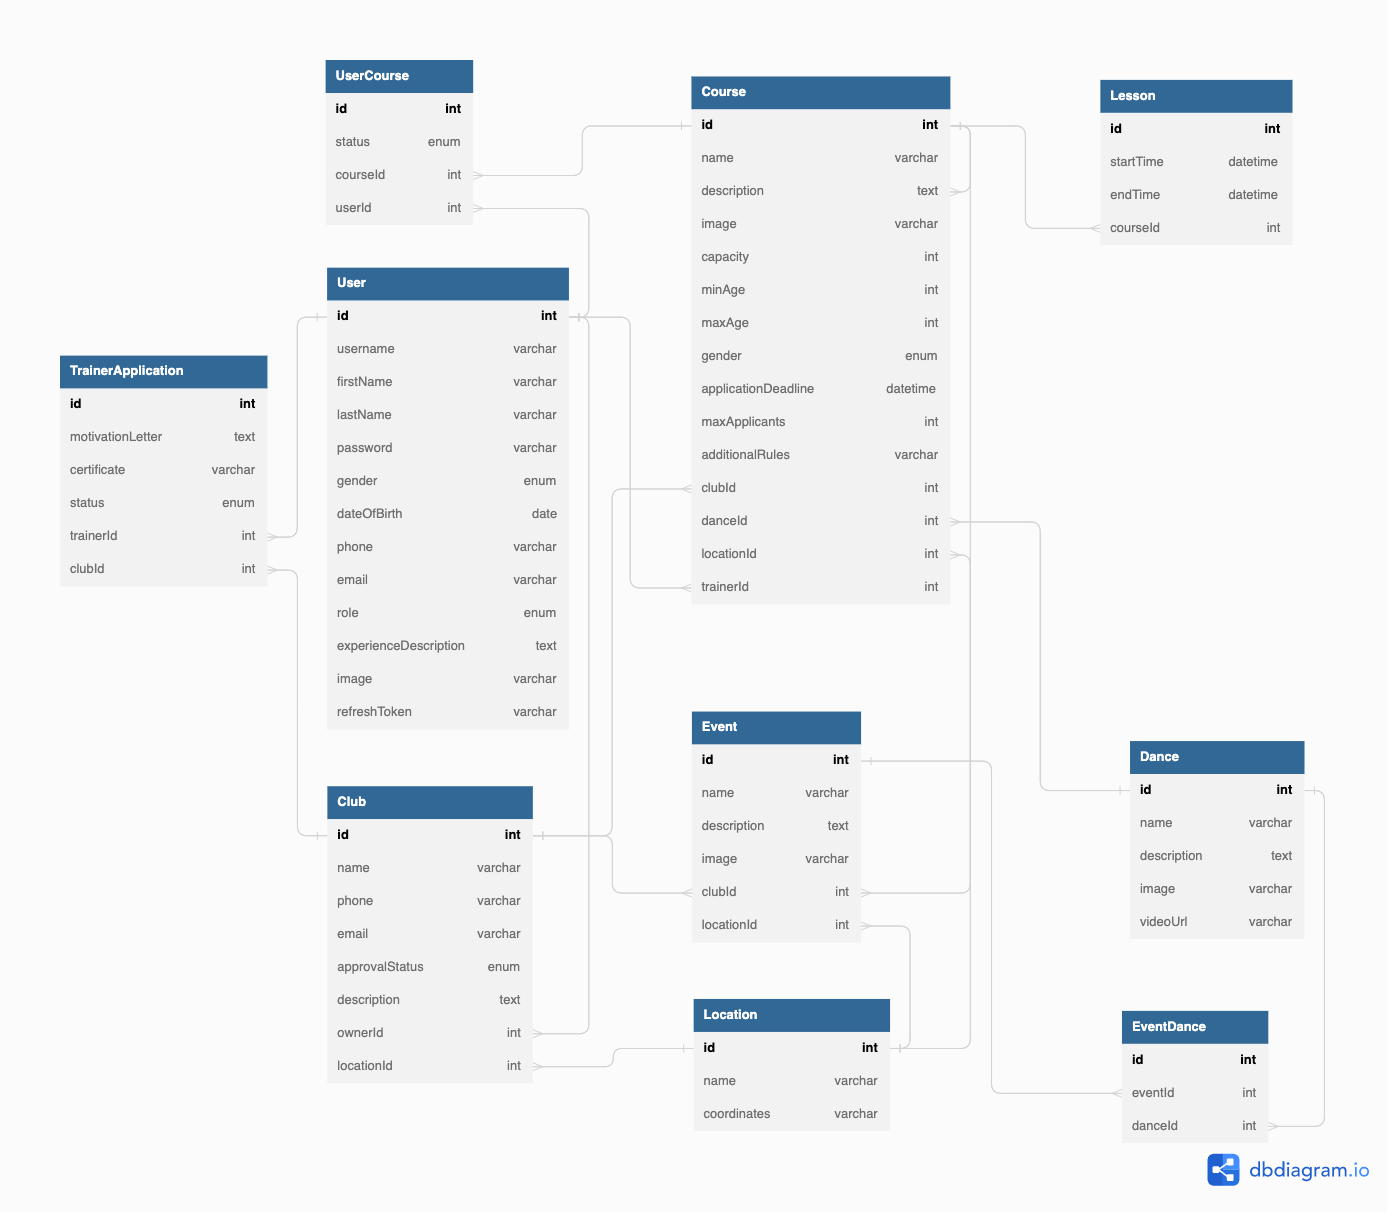
\includegraphics[scale=0.4]{slike/base_diagram.png}
			\centering
			\caption{Relacijski dijagram baze podataka.}
			\label{fig:promjene}
		\end{figure}
			
			\eject
			
			
		\section{Dijagram razreda}
		
			\textit{Potrebno je priložiti dijagram razreda s pripadajućim opisom. Zbog preglednosti je moguće dijagram razlomiti na više njih, ali moraju biti grupirani prema sličnim razinama apstrakcije i srodnim funkcionalnostima.}\\
			
			\textbf{\textit{dio 1. revizije}}\\
			
			\textit{Prilikom prve predaje projekta, potrebno je priložiti potpuno razrađen dijagram razreda vezan uz \textbf{generičku funkcionalnost} sustava. Ostale funkcionalnosti trebaju biti idejno razrađene u dijagramu sa sljedećim komponentama: nazivi razreda, nazivi metoda i vrste pristupa metodama (npr. javni, zaštićeni), nazivi atributa razreda, veze i odnosi između razreda.}\\
			
			\textbf{\textit{dio 2. revizije}}\\			
			
			\textit{Prilikom druge predaje projekta dijagram razreda i opisi moraju odgovarati stvarnom stanju implementacije}
			
			
			
			\eject
		
		\section{Dijagram stanja}
			
			
			\textbf{\textit{dio 2. revizije}}\\
			
			\textit{Potrebno je priložiti dijagram stanja i opisati ga. Dovoljan je jedan dijagram stanja koji prikazuje \textbf{značajan dio funkcionalnosti} sustava. Na primjer, stanja korisničkog sučelja i tijek korištenja neke ključne funkcionalnosti jesu značajan dio sustava, a registracija i prijava nisu. }
			
			
			\eject 
		
		\section{Dijagram aktivnosti}
			
			\textbf{\textit{dio 2. revizije}}\\
			
			 \textit{Potrebno je priložiti dijagram aktivnosti s pripadajućim opisom. Dijagram aktivnosti treba prikazivati značajan dio sustava.}
			
			\eject
		\section{Dijagram komponenti}
		
			\textbf{\textit{dio 2. revizije}}\\
		
			 \textit{Potrebno je priložiti dijagram komponenti s pripadajućim opisom. Dijagram komponenti treba prikazivati strukturu cijele aplikacije.}